\cotefile{63}
\scanpage{21}\mspage{6}
\[
\mathrm{u}^{4}\,\mathrm{c}'_{4}=\mathrm{c}_{4}\qquad
\mathrm{u}^{6}\,\mathrm{c}'_{6}=\mathrm{c}_{6}\qquad
\mathrm{u}^{12}\,\Delta'=\Delta\qquad.
\tag*{(1.8)}
\]

Les formules (1.8) expriment que la section $\mathrm{c}_{4}\,\pi^{\handwritten{\otimes}4}$ (resp. $\mathrm{c}_{6}\,\pi^{\handwritten{\otimes}6}$, resp. $\Delta\,\pi^{\handwritten{\otimes}12}$) du fibré $\omega^{\handwritten{\otimes}4}$ (resp. $\omega^{\handwritten{\otimes}6}$, $\omega^{\handwritten{\otimes}12}$)\raisebox{.35ex}{\tiny.} ne dépend pas du choix arbitraire de $\pi$, $\mathrm{x}$ et $\mathrm{y}$.
\par\noindent\hfill
\margin{\hspace{1.8cm}\makebox[0pt][r]{\begin{minipage}[t]{10.1cm}
\diagram{\handwritten{\raisebox{2.65\baselineskip}{\uline{Sur un corps}}\ \(\left\{\begin{array}{@{}l@{\quad}l@{}}
\text{Cas elliptique :}&\Delta\neq0\\
\text{cas multiplicatif :}&\Delta=0,\ \unsure{C|c}_{4}\neq0\ \text{(équiv.}\\[-.2ex]
&\hfill{\scriptstyle\unsure{c|e}}\\[-.3ex]
&\hspace{4em}\text{à }C_{6}\neq0)\\
\text{cas additif :}&\Delta=0,\ C_{4}=0\ \text{i.e.}\\
&\Delta=0,\ C_{6}=0
\end{array}\right.\)}}
\end{minipage}}}
\par\vspace{7.7\baselineskip}

2.\qquad \uline{Cas où 2 et 3 sont inversibles}.\margin{\handwritten{$\backslash$}}

Lorsque $2$ et $3$ sont inversibles, on peut d'une et d'une seule façon choisir $\mathrm{x}$ et $\mathrm{y}$ ($\pi$ étant donné) de sorte que dans l'équation (1.3.) on ait $\mathrm{a}_{1}=\mathrm{a}_{2}=\mathrm{a}_{3}=0$. On a alors
\[
\mathrm{y}^{2}=\mathrm{x}^{3}+\mathrm{a}_{4}\,\mathrm{x}+\mathrm{a}_{6}\qquad,\ \text{avec}\quad\pi=\mathrm{dx}/2\mathrm{y}\qquad,
\tag*{(2.1)}
\]
\[
\mathrm{c}_{4}=-2^{4}.3\mathrm{a}_{4}\quad,\quad
\mathrm{c}_{6}=-2^{5}.3^{3}\,\mathrm{a}_{6}\quad,\quad
\Delta=2^{4}(-4\mathrm{a}_{4}^{3}-27\,\mathrm{a}_{6}^{2})\quad.
\tag*{(2.2)}
\]

Posant $\mathrm{Y}=2\mathrm{y}$, $\mathrm{X}=\mathrm{x}$, on retombe sur la forme de Weierstrass
\[
\mathrm{Y}^{2}=4\,\mathrm{X}^{3}-\mathrm{g}_{2}\,\mathrm{X}-\mathrm{g}_{3}\quad,\ \text{avec}\quad\pi=\mathrm{d}\,\mathrm{X}/\mathrm{Y}\quad,\quad\text{et}
\tag*{(2.3)}
\]
\[
\begin{aligned}[t]
&\mathrm{g}_{2}=-4\,\mathrm{a}_{4}=\handwritten{\frac}{1}{12}\,\mathrm{c}_{4}\qquad
\mathrm{g}_{3}=-4\,\mathrm{a}_{6}=\handwritten{\frac}{1}{216}\,\mathrm{c}_{6}\\
&\Delta=\mathrm{g}_{2}^{3}-27\,\mathrm{g}_{3}^{2}\qquad.
\end{aligned}
\tag*{(2.4)}
\]

\uline{Proposition} 2.5.\quad \uline{Au dessus de} $\operatorname{Spec}(\handwritten{\mathbb{Z}}[2^{-1},\,3^{-1}]$, \uline{il existe un schéma de modules pour les courbes de genre un munies d'une forme différentielle invariante inversible}. \uline{C; schéma est}
\[
\operatorname{Spec}(\handwritten{\mathbb{Z}}[2^{-1},\,3^{-1}][\mathrm{g}_{2},\,\mathrm{g}_{3}]\qquad,
\]
\clearpage
% archive sheet number: 20
\scanpage{22}\mspage{7}
\uline{avec pour courbe universelle} (\uline{en coordonnées non homogò\`nos})
\[
\mathrm{Y}^{2}=4\,\mathrm{X}^{3}-\mathrm{g}_{2}\,\mathrm{X}-\mathrm{g}_{3}
\]
\margin{\handwritten{\uline{\unsure{section} unité} ?}}
\uline{et pour différentielle invariante} $\pi=\mathrm{d}\,\mathrm{X}/\mathrm{Y}$.

De plus, lorsque $2$ et $3$ sont inversibles, la donnée d'une forme différentielle invariante suffit à rigidifier une courbe de genre $1$.

Il résulte aussitôt de (2.2) qu'on a
\[
\mathrm{c}_{4}^{3}-\mathrm{c}_{6}^{2}=\underset{\inserted{\handwritten{12^{3}}}}{1728}\,\Delta
\tag*{(2.6)}
\]
et cette formule, se réduisant à une identité algébrique, est valable en toute caractéristique.

3.\qquad \uline{Cas où} $2$ \uline{et} $\mathrm{c}_{4}$ \uline{sont inversibles}.

Supposons que $\mathrm{E}$ soit une courbe de genre un sur une base $\mathrm{S}$ où $2$ soit inversible. La forme différentielle invariante $\pi$ étant donnée, on peut choisir $\mathrm{x}$ et $\mathrm{y}$ tels que dans (1.3) on ait $\mathrm{a}_{1}=\mathrm{a}_{3}=0$. Les changements de coordonnées respectant cette condition s'obtiennent en faisant $\mathrm{u}=1$, $\mathrm{s}=\mathrm{t}=0$ dans (1.2).

On a donc
\[
\mathrm{y}^{2}=\mathrm{x}^{3}+\mathrm{a}_{2}\,\mathrm{x}^{2}+\mathrm{a}_{4}\,\mathrm{x}+\mathrm{a}_{6}\,\raisebox{.14ex}{\scriptsize\unsure{,|'}}
\tag*{(3.1)}
\]
\[
\mathrm{b}_{2}=4\mathrm{a}_{2}\qquad\mathrm{b}_{4}=2\mathrm{a}_{4}\qquad
\mathrm{b}_{6}=4\mathrm{a}_{6}\qquad\mathrm{d}_{6}=8(\mathrm{a}_{2}\,\mathrm{a}_{4}-9\,\mathrm{a}_{6})
\]
\[
\mathrm{c}_{4}=2^{4}(\mathrm{a}_{2}^{2}-3\mathrm{a}_{4})\qquad
-\mathrm{c}_{6}=2^{6}\,\mathrm{a}_{2}^{3}-2^{5}\,3^{2}\,\mathrm{a}_{2}\,\mathrm{a}_{4}+2^{5}\,3^{3}\,\mathrm{a}_{6}\quad\text{et}
\tag*{(3.2)}
\]
\[
\Delta=2^{4}\,\delta\qquad,
\]
\clearpage
% archive sheet number: 21
\scanpage{23}\mspage{8}
où $\delta$ est le discriminant du second membre de (3.1). Le discriminant $\delta$ étant invariant par translation, il suffit de vérifier cette identité algébrique pour $3$ inversible et $\mathrm{a}_{2}=0$.

Lorsque $\mathrm{c}_{4}$ est inversible, un et un seul choix de $\mathrm{x}$ et $\mathrm{y}$ donne $\mathrm{d}_{6}=0$ ? i.e. $\mathrm{a}_{2}\,\mathrm{a}_{4}-9\,\mathrm{a}_{6}=0$. On a, lorsque cette condition est remplie,
\[
-\mathrm{c}_{6}=2^{6}(\mathrm{a}_{2}^{3}-3^{3}\,\mathrm{a}_{6})\qquad
\Delta=2^{6}(-\mathrm{a}_{2}^{3}\,\mathrm{a}_{6}-\mathrm{a}_{4}^{3}+2.3^{3}\,\mathrm{a}_{6}^{2})
\tag*{(3.3)}
\]
et
\[
\begin{aligned}[t]
\mathrm{a}_{2}\,\mathrm{c}_{4}&=-2^{-2}\,\mathrm{c}_{6}\\
\mathrm{a}_{4}\,\mathrm{c}_{4}^{2}&=-2^{2}\,3^{2}\,\Delta\\
\mathrm{a}_{6}\,\mathrm{c}_{4}^{3}&=\mathrm{c}_{6}\,\Delta\qquad.
\end{aligned}
\tag*{(3.4)}
\]

Il suffit de vérifier ces identités en caractéristique $0$, auquel cas la troisième est le produit des deux premières, puisque $\mathrm{d}_{6}=0$.

\uline{Proposition} 3.5.\quad \uline{Au dessus de} $\operatorname{Spec}(\handwritten{\mathbb{Z}}[2^{-1}])$, \uline{il existe un schéma de modul}\tikz[baseline=(ending.base)]{\node[inner sep=0pt] (ending) {\uline{e\handwritten{s}}};\handwritten{\draw[overlay,rotate around={-6:(ending.center)}] (ending.center) ellipse [x radius=.6em,y radius=1.35em];}}\uline{ pour les courbes de genre un munies d'une forme différentielle invariante inversible et telles que} $\mathrm{c}_{4}$ \uline{soit inversible. Ce schéma} \reversemarginpar\margin{\handwritten{\tikz[baseline=-.15ex]{\draw[thin,gray] (0,0) -- (.63em,.14em);}}}\normalmarginpar\uline{est}
\[
\operatorname{Spec}(\handwritten{\mathbb{Z}}[2^{-1}][\mathrm{a}_{2},\,\mathrm{a}_{4},\,\mathrm{a}_{6},\,(\mathrm{a}_{2}^{2}-3\,\mathrm{a}_{4})^{-1}]/(\mathrm{a}_{2}\,\mathrm{a}_{4}-9\,\mathrm{a}_{6}))
\]
\uline{avec pour courbe universelle} (\uline{en coordonnées non homogè}\tikz[baseline=(ending.base)]{\node[inner sep=0pt] (ending) {\uline{ne}\handwritten{s})};\handwritten{\draw[overlay] ([xshift=1.3em,yshift=2.16em]ending.center) .. controls +(-.8em,.42em) and +(.3em,1.1em) .. ([xshift=-.63em,yshift=.2em]ending.center) .. controls +(-.72em,-1.6em) and +(-.76em,-1.6em) .. ([xshift=1.35em,yshift=-.65em]ending.center) .. controls +(.7em,.8em) and +(.5em,1.6em) .. ([xshift=1.32em,yshift=2.22em]ending.center);}}
\[
\mathrm{y}^{2}=\mathrm{x}^{3}+\mathrm{a}_{2}\,\mathrm{x}^{2}+\mathrm{a}_{4}\,\mathrm{x}+\mathrm{a}_{6}
\]
\clearpage
% archive sheet number: 22
\scanpage{24}\mspage{9}
\uline{et pour différentielle invariante} $\pi=\mathrm{dx}/2\mathrm{y}$.

De plus, sous ces hypothèses, la donnée d'une forme différentielle invariante suffit à rigidifier une courbe.

4.\qquad \uline{Cas où} $2$ \uline{est nilpotent et} $\mathrm{c}_{4}$ \uline{inversible}.

Lorsque $2=0$, la forme différentielle ne suffit plus jamais à rigidifier une courbe de genre un. Lorsque $\mathrm{c}_{4}$ est inversible et $2$ nilpotent, donc $\mathrm{a}_{1}$ inversible, en changeant le choix de $\pi$, $\mathrm{x}$, $\mathrm{y}$ on peut trouver une équation
\[
\mathrm{y}^{2}+\mathrm{xy}=\mathrm{x}^{3}+\mathrm{a}_{2}\,\mathrm{x}^{2}+\mathrm{a}_{6}\qquad
\pi=\handwritten{\frac}{\mathrm{dx}}{\mathrm{x}+2\mathrm{y}}\qquad.
\tag*{(4.1)}
\]

Les autres choix de $\mathrm{x}$ et $\mathrm{y}$ donnant lieu à une telle équation s'obtiennent en faisant, dans (1.2)
\[
\mathrm{r}=\mathrm{t}=0\qquad\mathrm{u}=1+2\mathrm{s}
\tag*{(4.2)}
\]
et on aura
\[
\begin{aligned}[t]
\mathrm{u}^{2}\,\mathrm{a}'_{2}&=\mathrm{a}_{2}-\mathrm{s}-\mathrm{s}^{2}\\
\mathrm{u}^{6}\,\mathrm{a}'_{6}&=\mathrm{a}_{6}
\end{aligned}
\tag*{(4.3)}
\]
et \uline{modulo 2}
\[
\mathrm{c}_{4}=1\qquad\mathrm{c}_{6}=1\qquad\Delta=\mathrm{a}_{6}\qquad.
\tag*{(4.4)}
\]
\margin{\handwritten{\figure{\begin{tikzpicture}[x=1em,y=1em]
\draw[thin,gray] (0,1.15) -- (.72,1.12);
\draw[thin,gray] (.25,.85) -- (.25,.22);
\draw[thin,gray] (.88,.46) -- (.94,.57);
\draw[thin,gray] (.88,.23) -- (.93,.31);
\draw[thin,gray] (1.5,.43) .. controls (1.65,.68) and (1.82,.31) .. (2.08,.47);
\end{tikzpicture}}}}

5.\qquad \uline{Cas où} $\mathrm{c}_{4}=0$, $\mathrm{p}=2$ \uline{ou} $\mathrm{p}=3$\tikz[baseline=(mark.base)]{\node[inner sep=0pt] (mark) {.};\handwritten{\draw[overlay,thin,gray] ([xshift=.1em,yshift=.86em]mark.center) .. controls +(-.2em,.5em) and +(-.83em,-.8em) .. ([xshift=-.23em,yshift=-.9em]mark.center) .. controls +(.67em,-.12em) and +(0,-.45em) .. ([xshift=.93em,yshift=.5em]mark.center);}}\margin{\handwritten{\tikz[baseline]{\draw[thin,gray] (0,0) .. controls (.12em,.38em) and (.38em,.27em) .. (.58em,.25em);}}}

a) $\mathrm{p}=3$

En caractéristique $3$, lorsque l'équation est mise sou\tikz[baseline=(ending.base)]{\node[inner sep=0pt] (ending) {s};\node[overlay,inner sep=0pt,anchor=base] at (ending.base) {\deleted{r}};\handwritten{\draw[overlay,thin,gray] ([xshift=-.1em,yshift=.85em]ending.center) .. controls +(-.35em,.32em) and +(-.45em,.82em) .. ([xshift=-.67em,yshift=-.05em]ending.center) .. controls +(.2em,-1em) and +(.8em,-.48em) .. ([xshift=.59em,yshift=-.1em]ending.center) .. controls +(0,.75em) and +(.42em,.34em) .. ([xshift=-.1em,yshift=.55em]ending.center);}} forme
% archive sheet number: 23
\scanpage{25}
\mspage{10}

(3.1), $c_4=0$ si et seulement si $a_2^2=0$. Supposons qu'on ait même $a_2=0$
\[
\begin{aligned}[t]
 &y^2=x^3+a_4 x+a_6 \qquad \pi=a_4^{-1}\,dy=dx/2y\\[.65em]
 &c_4=c_6=0 \qquad \Delta=-a_4^3 \, .
\end{aligned}\tag*{(5.1)}
\]

Les autres systèmes $(\pi,x,y)$ donnant une équation de cette forme s'obtiennent en faisant $s=t=0$ dans (1.2) et
\[
\begin{aligned}
u^4 {\mathbb{\text{\makebox[0pt][l]{\kern.45pt$a$}$a$}}}'_4 &= a_4\\
u^6 a'_6 &= a_6+r\,a_4+r^3 \, .
\end{aligned}\tag*{(5.2)}
\]

b) $p=2$\tikz[baseline=(p.base)]{\node[inner sep=0pt] (p) {.};\handwritten{\draw[thin,gray] (0.13em,1.1em) .. controls (-0.42em,1.25em) and (-0.57em,-1.52em) .. (-0.01em,-1.45em) .. controls (0.40em,-1.46em) and (0.77em,0.33em) .. (0.75em,1.44em);}}

En caractéristique 2 , on a $c_4=a_1^4$. Supposons qu'on ait $a_1=0$ ; $\pi$ étant donnée, on peut alors choisir $x$ et $y$ tels que (1.3) soit
\[
\begin{aligned}[t]
 &y^2+a_3\,y=x^3+a_4\,x+a_6 \qquad
\pi=\frac{dx}{a_3}=dy/\tikz[baseline=(den.base)]{\node[inner sep=0pt] (den) {$x^2+a_4$};\handwritten{\draw[<->,thin] ([yshift=0.6ex]den.north west) .. controls ([xshift=-0.3em,yshift=-1.1ex]den.south west) and ([xshift=-0.1em,yshift=-1.1ex]den.south east) .. ([xshift=0.32em,yshift=-0.35ex]den.south east) .. controls ([xshift=0.6em]den.south east) and ([xshift=0.32em]den.north east) .. ([xshift=0.32em,yshift=0.65ex]den.north east);}}
\\[.65em]
 &b_2=b_4=0 \qquad b_6=a_3^2 \qquad b_8=a_4^2 \qquad
\Delta=a_3^4 \qquad c_4=c_6=0 \, .
\end{aligned}\tag*{(5.3)}
\]

Les autres systèmes $(\tikz[baseline=(pc.base)]{\node[inner sep=0pt] (pc) {$\pi,$};\handwritten{\draw[thin,gray,rotate around={-9:(pc.center)}] (pc.center) ellipse (0.62em and 1.07em);}}\,x,y)$ donnant une équation de cette forme s'obtiennent en faisant $r=s^2$ dans (1.2) et
\[
\begin{aligned}
u^3 a'_3 &= a_3\\
u^4 a'_4 &= a_4+sa_3+s^4\\
u^6 a'_6 &= a_6+s^2\,a_4+ta_3+s^6+t^2 \, .
\end{aligned}\tag*{(5.4)}
\]
% archive sheet number: 24
\scanpage{26}
\mspage{11}

6. \quad \uline{Applications}.

\uline{Proposition} 6.1. \quad \uline{Si} $E$ \uline{est une courbe de genre un sur un corps algébriquement clos}, $E$ \uline{est de type elliptique} (\uline{resp. multiplicatif}, \uline{resp. additif}) \uline{si et seulement si} $\Delta\ne 0$ (\uline{resp.} $\Delta=0$ et $c_4\ne 0$, \uline{resp}. $\Delta=c_4=0$).

a) \quad Lorsque la caractéristique $p\ne 2$, la première assertion résulte de la troisième formule (3.2). Lorsque $p=2$ et $c_4\ne 0$, on vérifie aussitôt que la différentielle de (4.1) ne s'annule qu'en $(0,0)$, et $\Delta$ est elliptique si et seulement si $\Delta=a_6\ne 0$. Pour $p=2$ et $c_4=0$, on raisonne de même sur (6.2).

b) \quad Lorsque $p\ne 2$, il résulte de (3.2) que $\Delta=c_4=0$ si et seulement si le deuxième membre de (3.1) a toutes ses racines égales, ce qui caractérise le cas additif.

c) \quad Lorsque $p=2$, $\Delta=0$, $c_4\ne 0$, la partie principale de (4.1) en $(0,0)$ est $y^2+xy+a_2x^2=0$, ce qui correspond à un point double à tangentes distinctes.

d) \quad Lorsque $p=2$, $\Delta=0$, $c_{4.}=0$, la partie principale de (6.2) en $(0,0)$ est $y^2+a_4x+a_6=0$, ce qui correspond à une singularité cuspidale.

Soit alors $E$ une courbe de genre un sur une base $S$, sans fibre de type additif. Puisque $\Delta$ et $\unsure{\mathbb{\text{\makebox[0pt][l]{\kern.45pt$c$}$c$}}_4|c_4}$ ne sont jamais simultanément nuls, et sont respectivement des sections de $\omega^{\otimes 12}$ \tikz[baseline=(et.base)]{\node[inner sep=0pt] (et) {et};\handwritten{\draw[thin,gray,rotate around={-27:(et.center)}] (et.center) ellipse (0.80em and 1.16em);}} $\omega^{\otimes 4}$, on définit une section $j$ de
$\tikz[baseline=(P.base)]{\node[inner sep=0pt] (P) {$P_1$};\handwritten{\draw[thin,gray,rotate around={-16:(P.center)}] (P.center) ellipse (0.90em and 1.24em);}\node[inner sep=0pt,below=0.95em] (corr) at (P.south) {\inserted{\handwritten{$P^1$}}};\handwritten{\draw[thin,gray,rotate around={-21:(corr.center)}] (corr.center) ellipse (1.08em and 1.29em);}}/S$
par la formule%
% archive sheet number: 25
\scanpage{27}%
\mspage{12}%
\margin{\handwritten{$\begin{aligned}j&=0 &&\Longleftrightarrow c_4=0\\j&=12^3 &&\Longleftrightarrow c_6=0\end{aligned}$}}%
\[
j=c_4^3/\Delta=1728+c_6^2/\Delta \, . \tag*{(6.2)}
\]

\uline{Proposition} 6.3. \quad \uline{Soient} $E$ \uline{et} $E'$ \uline{deux courbes de genre un sur} $S$, \uline{sans fibre additive} .

(I) $\text{\uline{Isom}}_{\handwritten{S}}(E,E')$ \uline{est représentable, fini et} \tikz[baseline=(nrone.base)]{\node[inner sep=0pt] (nrone) {\uline{non ramifié}};\handwritten{\draw[thin,gray] (nrone.north east) .. controls ([xshift=-1em,yshift=0.8em]nrone.north east) and ([xshift=-0.6em,yshift=0.7em]nrone.north west) .. ([xshift=-0.2em]nrone.west) .. controls ([yshift=-0.85em]nrone.south west) and ([xshift=0.5em,yshift=-0.85em]nrone.south east) .. (nrone.north east);}\node[anchor=south west,inner sep=0pt] at ([xshift=-1.8em,yshift=0.48em]nrone.north east) {\inserted{\handwritten{net}}};} \uline{sur} $S$\tikz[baseline=(stop.base)]{\node[inner sep=0pt] (stop) {.};\handwritten{\draw[thin] ([yshift=-0.08em]stop.south) .. controls ([xshift=0.04em,yshift=-0.19em]stop.south) .. ([xshift=-0.15em,yshift=-0.35em]stop.south);\draw[thin,gray,rotate around={-18:(stop.center)}] (stop.center) ellipse (0.56em and 1.34em);}}

(II) \uline{si} $j_E=j_F$, \uline{la projection de} $\text{\uline{I\mbox{$\mathbb{\text{\makebox[0pt][l]{\kern.45pt$s$}$s$}}$}om}}_{\handwritten{S}}(E,E')$ \uline{sur} $S$ \uline{est surjective}\tikz[baseline=(stop.base)]{\node[inner sep=0pt] (stop) {.};\handwritten{\draw[thin] ([yshift=-0.08em]stop.south) .. controls ([xshift=0.04em,yshift=-0.19em]stop.south) .. ([xshift=-0.15em,yshift=-0.35em]stop.south);\draw[thin,gray,rotate around={-18:(stop.center)}] (stop.center) ellipse (0.56em and 1.34em);}}

(III) \uline{si} $j_E=j_F$ \uline{ne prend pas les valeurs} $0$ \uline{et} $\underset{\inserted{\handwritten{\substack{\Vert\\12^3}}}}{\tikz[baseline=(val.base)]{\node[inner sep=0pt] (val) {$1728$};\handwritten{\draw[thin] (val.south west) .. controls ([yshift=-0.15em]val.south west) and ([yshift=-0.15em]val.south east) .. (val.south east);}}}$, $\text{\uline{Isom}}_{\handwritten{S}}(E,E')$ \uline{est un revêtement étale de rang} $2$ \uline{de} $S$ .

Donnons-nous $E$ et $E'$ par des équations (1.3) et $(1.3)'$. Se donner un isomorphisme entre $E$ et $E'$ revient à se donner $u$, $r$, $s$ et $t$, vérifiant les équations (1.6), donc aussi (1.7) et (1.8), $u$ devant de plus être inversible. Par hypothèse, localement sur $S$, $c_4$ ou $\Delta$ est inversible (6.1), et de même $c'_4$ ou $\Delta'$ l'est. Localement sur $S$, les équations (1.8) sont donc des équations de dépendance intégrale pour $u$ et $u^{-1}$, les équations $(1.7)_6$ ou $(1.7)_8$ des équations de dépendance intégrale pour $r$ et enfin $(1.6)_6$ (resp. $(1.6)_2$) est une équation de dépendance intégrale pour $t$ (resp. $s$). Ceci prouve que $\text{\uline{Isom}}(E,E')$ est représentable par un schéma affine fini sur $S$ ; il est même \tikz[baseline=(nrtwo.base)]{\node[inner sep=0pt] (nrtwo) {non ramifié};\handwritten{\draw[thin,gray] (nrtwo.north east) .. controls ([xshift=-1em,yshift=0.8em]nrtwo.north east) and ([xshift=-0.6em,yshift=0.7em]nrtwo.north west) .. ([xshift=-0.2em]nrtwo.west) .. controls ([yshift=-0.85em]nrtwo.south west) and ([xshift=0.5em,yshift=-0.85em]nrtwo.south east) .. (nrtwo.north east);}\node[anchor=south west,inner sep=0pt] at ([xshift=-1.8em,yshift=0.48em]nrtwo.north east) {\inserted{\handwritten{net}}};} car les courbes considérées n'ont pas d'automorphismes infinitésimaux (respectant l'origine).

Lorsque $2$ est inversible sur $S$, l'assertion (III) résulte de l'énoncé plus précis.

\uline{Proposition} 6.4. \quad \uline{Soient} $E$ \uline{et} $E'$ \uline{deux courbes de genre un sur} $S$ ,%
% archive sheet number: 26
\scanpage{28}%
\mspage{13}\space
\uline{sans fibre additive}, \uline{munies de formes différentielles invariantes} $\pi$ \uline{et} $\pi'$, \uline{et de même invariant modulaire}. \uline{On suppose que} $2$, $c_4$ \uline{et} $c_6$ \uline{sont inversibles}, \uline{i.e.} \uline{que} $2^{-1}$, $1/j$ et $1/\inserted{\handwritten{(}}j-1728\inserted{\handwritten{)}}$ \uline{sont des sections de} \tikz[baseline=(ess.base)]{\node[inner sep=0pt] (ess) {$S$};\handwritten{\draw[thin,gray,rotate around={-20:(ess.center)}] (ess.center) ellipse (0.52em and 1.02em);}}\reversemarginpar\margin{\inserted{\handwritten{\tikz[baseline=(oh.base)]{\node[inner sep=0pt] (oh) {$\underline{O}_S$};\handwritten{\draw[thin,gray,rotate around={-15:(oh.center)}] (oh.center) ellipse (1.13em and 1.55em);}}}}}\normalmarginpar. \uline{Alors}, \uline{le schéma} $\text{\uline{Isom}}(E,F)$ \uline{s'identifie au schéma défini par l'équation}
\[
\lambda^2=c_4\,c'_6/c_6\,c'_4 \, .
\]

En vertu de (3.6), se donner $(E,\pi)$ revient à se donner $a_2$, $a_4$ et $a_6$ vérifiant $a_2\,a_4-9\,a_6=0$, et un isomorphisme de $E$ sur $E'$ est décrit par $\lambda$ tel que $(E\,\pi)$ soit isomorphe à $(E',\lambda\,\pi')$, i.e. par $\lambda$ vérifiant
\[
a'_2=\lambda^2\,a_2 \qquad a'_4=\lambda^4\,a_4 \qquad a'_6=\lambda^6\,a_6 \, . \tag*{(6.4.1)}
\]

Par hypothèse, $j=j'$, de sorte que $(c_4^3,c_6^2,\Delta)$ est proportionnel à $(c_4^{\raisebox{-.38ex}{$\scriptstyle\prime$}\,3},c_6^{\raisebox{-.38ex}{$\scriptstyle\prime$}\,2},\Delta')$, et que $\mu=c_4\,c'_6/\raisebox{-.52ex}{$c_6\,c'_4$}$ vérifie
\[
c'_4=\mu^2\,c_4 \qquad c'_6=\mu^3\,c_6 \qquad \Delta'=\mu^6\,\Delta \, . \tag*{(6.4.2)}
\]

En vertu de (3.4), on a alors
\[
{\mathbb{\text{\makebox[0pt][l]{\kern.45pt$a$}$a$}}}'_2=\mu\,a_2 \qquad a'_4=\mu^2\,a_4 \qquad a'_6=\mu^3\,a_6 \, .
\]

De plus, d'après (3.4) encore, localement, soit $a_2$, soit $a_4$ et $a_6$ sont inversibles, de sorte que (6.4.1) équivaut à $\lambda^2=\mu$.

Pour prouver (III) en général, on peut se ramener à supposer $S$ noethérien, et supposer soit $2$ inversible (cas traité en (6.4)), soit%
% archive sheet number: 27
\scanpage{29}%
\mspage{14}\space
$2$ nilpotent, ce qui permet de mettre la courbe sous la forme (4.1)
\[
y^2+xy=x^3+a_2\,x+a_6
\]
et un isomorphisme d'une telle courbe sur une autre est décrit par $s$ vérifiant (4.3) pour $u=1+2s$. Lorsque $j=j'$, la première de ces équations
\[
(1+2s)^2\,a'_2=a_2-s-s^2
\]
définit un revêtement étale de degré deux, et elle implique la seconde ; pour le voir, on se ramène à supposer $a_2=a'_2$ et on remarque que d'après (4.4)
\[
1/j=a_6+2\,R(a_2,a_6)
\]
pour une fraction rationnelle $R$ .

Pour vérifier (II) dans les cas non couverts par (III), on peut supposer que $S$ est le spectre d'un corps algébriquement clos et que $c_4=0$ ou $c_6=0$ \tikz[baseline=(punct.base)]{\node[inner sep=0pt] (punct) {,};\node[inner sep=0pt,anchor=north] at ([yshift=-0.16em]punct.south) {.};} i.e. que $j=0$ ou $j=1728$. Soit $p$ la caractéristique du corps,

a) $p\ne 2,3$ : on met la courbe sous la forme (2.1) ; si $c_4=0$ (resp. $c_6=0$) on aura $a_4=0$ (resp. $a_6=0$) et on peut par homothétic transformer la courbe en la courbe type
\[
y^2=x^3+1 \qquad (\text{si }c_4=0) \tag*{(6.5)}
\]
\[
y^2=x^3-x \qquad (\text{si }c_6=0) \tag*{(6.6)}
\]

b) $\unsure{\mathbb{\text{\makebox[0pt][l]{\kern.45pt$p$}$p$}}|p}=3$ : on met la courbe sour la forme (6.1) ; résolvant (6.2) pour $a'_4=1$ et $a'_6=0$, on met la courbe sous la forme type%
% archive sheet number: 28
\scanpage{30}%
\mspage{15}%
\[
y^2=x^3-x \qquad (\text{si }c_4=c_6=0) \tag*{(6.7)}
\]

c) $p=2$ : ici, on met la courbe sour la forme (6.3) et on résoud (6.4) avec $a_3\unsure{\cdot}=1$, $a_4=a_6=0$ pour obtenir la forme type
\[
y^2+y=x^3 \qquad (\text{si }c_4=c_6=0) \, . \tag*{(6.8)}
\]

Pour compléter le tableau, reste à décrire les automorphismes des courbes elliptiques.

\uline{Proposition} 6.9. \quad \uline{Soit} $E$ \uline{une courbe de genre un sur une base} $S$, \uline{sans fibre additive}.

(I) \quad \uline{Si} $c_4$ et $c_6$ \uline{sont inversibles,} \uline{les seuls automorphismes}\margin{\tikz[baseline=(rem.base)]{\node[align=left,inner sep=2pt] (rem) {\handwritten{faux si $S$}\\\handwritten{\unsure{pas} connexe}};\handwritten{\draw[thin,gray,rounded corners=4pt] (rem.north east) -- (rem.south east) -- (rem.south west) -- (rem.north west) -- ([xshift=-0.4em]rem.north east);\draw[thin] ([xshift=0.35em,yshift=0.5em]rem.north west) -- ([xshift=0.2em]rem.west);}}} \uline{de} $E$ \uline{sont l'identité et la symétrie}.

(II) \quad \uline{Si} $2$ et $3$ \uline{sont inversibles}, \uline{l'application canonique}
\diagram{\[
\vcenter{\hbox{\begin{tikzcd}[ampersand replacement=\&,column sep=1.9em]
 \text{\uline{Aut}}(E) \handwritten{\arrow[r]} \& G_m
\end{tikzcd}}}\tag*{(6.6.)}
\]}
\uline{donnée par l'action sur les différentielles invariantes}, \uline{est une immersion fermée}.

(III) \uline{Si} $2$ \uline{et} $3$ \uline{sont inversibles}, \uline{et} $c_4=0$ (resp. $c_6=0$) \uline{l'image de} (6.6) \uline{est} $\mu_6$ (resp. $\mu_4$).

\uline{Supposons maintenant que} $S$ \uline{soit le spectre d'ur corps}\tikz[baseline=(stop.base)]{\node[inner sep=0pt] (stop) {.};\handwritten{\draw[thin,gray,rotate around={-18:(stop.center)}] (stop.center) ellipse (0.57em and 1.03em);}}

(IV) \quad \uline{Si} $3=c_4=c_6=0$, $\mathrm{Aut}(E)$ \uline{est géométriquement \unsure{isomorphe} au produit semi-direct} (\uline{non commutatif}) \uline{de} $\mathbb{Z}/(4)$ \uline{par} $\mathbb{Z}/(3)$, \uline{et l'image de} (6.6) \uline{est} $\mu_4$ .

(V) \quad \uline{Si} $2=c_4=c_6=0$, $\mathrm{Aut}(E)$ \uline{est géométriquement d'ordre} \tikz[baseline=(order.base)]{\node[inner sep=0pt] (order) {$24$,};\handwritten{\draw[thin,gray,rotate around={-38:(order.center)}] ([xshift=.37em,yshift=2.08em]order.center) arc[start angle=72,end angle=365,x radius=1.19em,y radius=2.2em];}}\margin{\handwritten{\tikz[baseline=-0.3ex]{\draw[thin] (0,0.7em) -- (0.35em,-0.05em);} structure ?}} \uline{et l'image de} (6.6) \uline{est} $\mu_3$.
% archive sheet number: 29
\scanpage{31}
\mspage{16}

\uline{Preuve} : (I) \quad D'après (6.3), il n'y a en effet pas plus de deux automorphismes.

(II) et (III) \quad Lorsque les courbes sont mises sous la forme (2.1), il résulte de (2.5) que les automorphismes sont décrits parleur action sur $\pi$ et que $\lambda\in G_m$ défini un automorphisme si et seulement si
\[
c_4=\lambda^4\,c_4 \qquad\text{et}\qquad c_6=\lambda^6\,c_6 \, ,
\]
d'où les assertions.

(IV) \quad Si la courbe est mise sous forme (6.1), les automorphismes sont donnés par (1.2) : $x'\handwritten{\mathrel{\tikz[baseline=-.32ex]{\draw[->,thin] (0,0) .. controls (.19em,.39ex) and (.28em,.6ex) .. (.57em,.18ex) .. controls (.78em,-.23ex) and (1.02em,-.08ex) .. (1.28em,0) -- (2.28em,.04ex);}}}x$, pour $s=t=0$ et
\[
\handwritten{\left\{}\begin{aligned}
&u^4=1\\
&r^3+ra_4+a_6(1-u^2)=0
\end{aligned}\right.
\]
et la loi de composition par
\[
(u',r')\quad (u,r)=(u\,u',u^{\raisebox{-.38ex}{$\scriptstyle\prime$}\,2}r+r')
\]

Lorsque la courbe est mise sous forme (6.7), ces équations se réduisent à $u\in\mu_4$ et $r\in F_3$ .

(V) \quad Si la courbe est mise sous forme (6.3), les automorphismes sont donnés par (1.2) : $x'\handwritten{\mathrel{\tikz[baseline=-.32ex]{\draw[->,thin] (0,0) .. controls (.14em,.37ex) and (.25em,.52ex) .. (.44em,.13ex) .. controls (.62em,-.25ex) and (.86em,-.2ex) .. (1.09em,.08ex) .. controls (1.3em,.31ex) and (1.52em,.23ex) .. (1.67em,.20ex) -- (2.36em,.16ex);}}}x$, pour $r=s^2$ et
\[
\handwritten{\left\{}\begin{aligned}
&u^3=1\\
&s^4+sa_3+a_4(1-u)=0\\
&t^2+ta_3+s^6+s^2\,a_4=0
\end{aligned}\right.
\]%
% archive sheet number: 30
\scanpage{32}%
\mspage{17}%
et la loi de composition par
\[
(u',s',t')\mathbin{\handwritten{o}}(u,s,t)
=(u\,u',u's+t',u^{\raisebox{-.38ex}{$\scriptstyle\prime$}\,3}t+t'+u^{\raisebox{-.38ex}{$\scriptstyle\prime$}\,2}rs')\, .
\]

Lorsque la courbe est mise sous forme (6.8), ces équations se réduisent à
\[
\begin{aligned}
u\in\mu_3 \qquad s\in\mathbb{F}_4 \qquad t^2+t=s^3
 &\quad ({}=0\ \text{ou}\ 1\ \text{selon que}\\
 &\qquad s=0\ \text{ou}\ s\ne 0) \, .
\end{aligned}
\]

7. \quad \uline{Anneau des formes modulaires entières}.

On appelle forme modulaire entière de poids $n$ une loi qui à chaque courbe de genre un sur une base $S$ associe une section de $\omega^{\otimes n}$, et ce de façon compatible au changement de base. Il reviendrait\margin{\handwritten{\tikz[baseline=-0.2ex]{\draw[thin,gray] (0,-0.35em) -- (0.48em,1.30em);} \uuline{pourquoi} ?}} au même de se limiter aux courbes sans fibres additives.

\uline{Proposition} 7.1. \quad \uline{L'anneau des formes modulaires entières est engendré sur} $\mathbb{Z}$ \uline{par} $c_4$, $c_6$ \uline{et} $\Delta$ \uline{soumis à la seule relation}
\[
c_4^3-c_6^2=1728\,\Delta \, . \tag*{(7.2.)}
\]
\margin{\tikz[baseline=(note.north)]{\node[inner sep=2pt,text width=9.8em,align=left] (note) {\handwritten{N.B. Sur le site modulaire, les diviseurs de $c_4$, $c_6$, $\Delta$ sont à \unsure{multiplicité|multiplicités} $1$ ; Celui de $\Delta$ est lisse sur $\mathbb{Z}$, ceux de $c_4$, $c_6$ le sont sauf au dessus des points $2$ et $3$.}};\handwritten{\draw[thin,rounded corners=1pt] (note.north west) -- (note.south west) -- (note.south east);}}}

Appliquant la définition à la courbe (1.3), on voit qu'une forme modulaire entière de poids $n$ s'exprime comme poly\tikz[baseline=(nome.base)]{\node[inner sep=0pt] (nome) {nôme};\handwritten{\draw[thin,gray,rotate around={-25:(nome.center)}] (nome.center) ellipse (1.04em and 1.65em);}} de poids $n$ en les $a_i$. Pour $2$ et $3$ inversibles, il résulte de 2.5 que ces formes sont \tikz[baseline=(des.base)]{\node[inner sep=0pt] (des) {des};\handwritten{\draw[thin,gray,rotate around={-15:(des.center)}] (des.center) ellipse (1em and 1.02em);}} poly\tikz[baseline=(noms.base)]{\node[inner sep=0pt] (noms) {nôm};\handwritten{\draw[thin,gray,rotate around={-25:(noms.center)}] (noms.center) ellipse (0.84em and 1.47em);}}es en $c_4$ et $c_6$, et en particulier que $c_4$, $c_6$ et $\Delta$ ne satisfont pas d'autres relations que (7.2). Reste à prouver que si un poly\tikz[baseline=(nomt.base)]{\node[inner sep=0pt] (nomt) {nôme};\handwritten{\draw[thin,gray,rotate around={-25:(nomt.center)}] (nomt.center) ellipse (0.85em and 1.53em);}} en $c_4$, $c_6$ et $\Delta$ est identiquement nul en caractéristique $2$ (resp. $3$), alors il est divisible par $2$ (resp.$3$) dans $\mathbb{Z}[c_4,c_6,\Delta]/\handwritten{\bigl(}c_4^3-c_6^2-1728\,\Delta\handwritten{\bigr)}$, ce qui signifie%
% archive sheet number: 31
\scanpage{33}%
\mspage{18}\space
qu'il est divisible par $c_4^3-c_6^2$ dans $\mathbb{Z}/(2)[c_4,c_6,\Delta]$ (resp. $\mathbb{Z}/(3)[c_4,c_6,\Delta]$). Cela résulte de la structure de l'anneau des formes modulaires de caractéristique $2$ (resp. $3$).

\uline{Proposition} 7.2. \quad (I) \uline{L'anneau des formes modulaires de caractéristique} $2$ \uline{est} $\mathbb{Z}/(2)[\tikz[baseline=(coeffa.base)]{\node[inner sep=0pt] (coeffa) {$a_1$};\handwritten{\node[inner sep=0pt,anchor=west,font=\scriptsize] (notea) at ([xshift=1.35em,yshift=-1.05em]coeffa.south west) {le diviseur de $a_1$ est lisse sur $\mathbb{F}_2$};\draw[thin] (coeffa.south west) to[out=-86,in=192] ([xshift=-.18em]notea.west);}\pgfresetboundingbox\path[use as bounding box] ([yshift=-1.5em]coeffa.south west) rectangle (coeffa.north east);},\Delta]$ , \uline{et} $c_4=a_1^4$ , $c_6=a_1^6$ .

\hspace*{3em}(II) \uline{L'anneau des formes modulaires de caractéristique} $3$ \uline{est} $\mathbb{Z}/(3)[\tikz[baseline=(coeffb.base)]{\node[inner sep=0pt] (coeffb) {$b_2$};\handwritten{\node[inner sep=0pt,anchor=west,font=\scriptsize] (noteb) at ([xshift=1.35em,yshift=-1.05em]coeffb.south west) {le diviseur de $b_2$ est lisse sur $\mathbb{F}_2$};\draw[thin] (coeffb.south west) to[out=-86,in=192] ([xshift=-.18em]noteb.west);}\pgfresetboundingbox\path[use as bounding box] ([yshift=-1.5em]coeffb.south west) rectangle (coeffb.north east);},\Delta]$ , et $c_4=b_2^2$ , $c_6=-b_2^3$ .

Tout d'abord, il résulte de $(1.6)_1$ et $(1.7)_2$ que $a_1$ (resp. $b_2$) est une forme modulaire de caractéristique $2$ (resp. $3$) .

En caractéristique $2$ , cherchons tout d'abord les formes modulaires relatives aux seules courbes telles que $a_1$ soit inversible. Ces courbes se mettent sous forme (cf. (4.\tikz[baseline=(un.base)]{\node[inner sep=0pt] (un) {1};\handwritten{\draw[thin,gray,rotate around={-12:(un.center)}] (un.center) ellipse (0.36em and 1.12em);}}))
\[
 y^2+a_1xy=x^3+a_2x^2+a_6 \qquad \pi=\frac{dx}{a_1x}
\]
et, compte tenu de (4.3), on voit que ces formes s'écrivent
\[
\begin{aligned}
 &a_1^{-n}\,P(a_1,a_6) \qquad \text{pour }P\text{ isobare, ou encore}\\[.65em]
 &a_1^{-m}\,Q(a_1,\Delta)\quad\handwritten{,}
\end{aligned}
\]
et cela garde un sens pour $a_1=0$ , $\Delta\ne0$ si et seulement si on avait en fait affaire à un polyn\tikz[baseline=(oc.base)]{\node[inner sep=0pt] (oc) {ô};\handwritten{\draw[thin,gray,rotate around={-14:(oc.center)}] (oc.center) ellipse (0.56em and 1.1em);}}me en $a_1$ et $\Delta$ .

En caractéristique $3$ , raisonnant de même d'abord sur les courbes telles que $c_4$ soit inversible, et remarquant que $d_6=0$ équivaut alors à $a_4=0$ dans (3.1), on voit que toute forme modu%
% archive sheet number: 32
\scanpage{34}%
\mspage{19}%
laire s'écrit
\[
 b_2^{-n}\,P(b_2,\Delta) \qquad \text{pour }P\text{ isobare}\quad ,
\]
et que cette forme modulaire est définie aussi pour $j=0$ si et seulement si elle s'écrit comme polyn\tikz[baseline=(oend.base)]{\node[inner sep=0pt] (oend) {ô};\handwritten{\draw[thin,gray,rotate around={-20:(oend.center)}] (oend.center) ellipse (0.64em and 1.15em);}}me en $b_2$ et $\Delta$ .

\handwritten{Interpr\unsure{é|e}tation de $a_1$, $b_2$ comme forme de Hasse-Witt ?}

\handwritten{Formes modulaires \unsure{sur|en} un corps quelconque ? Sur un ann. de val. discrète\ldots}

\handwritten{Hasse-Witt sur un corps de car $p>0$ quelconque ?}

\noindent\handwritten{\tikz{\draw[thin] (0,0) -- (3em,.06em);}}

\[
\handwritten{\left\{\begin{aligned}
 &\text{Relèvement canonique de Serre par formules universelles}\,\big|\\
 &\text{Loi de groupe formel sur }{\mathcal{P}}^{\infty}_{M/S}\ \text{: formules explicites\ldots}
\end{aligned}\right.}
\]
% archive sheet number: 33
\scanpage{41}
\noindent\hfill atkin \mspage{1}\margin{\handwritten{\figure{
\begin{tikzpicture}[x=.33mm,y=-.33mm,line cap=round,line join=round]
\draw (4,18) .. controls (12,7) and (21,4) .. (22,5) .. controls (19,11) and (13,16) .. (12,18);
\draw (15,13) .. controls (23,6) and (38,-2) .. (39,1) .. controls (38,8) and (27,26) .. (19,34) .. controls (15,39) and (12,39) .. (12,34);
\draw (13,9) .. controls (-3,24) and (-2,34) .. (11,31) .. controls (22,29) and (29,26) .. (19,24) -- (6,22);
\draw (12,29) .. controls (3,41) and (2,46) .. (8,42) .. controls (14,40) and (28,22) .. (38,22) .. controls (48,22) and (21,41) .. (6,51) .. controls (-1,61) and (20,40) .. (77,30);
\draw (33,18) -- (35,36);
\fill (47,34) circle (.55);
\end{tikzpicture}}}}

\begin{center}
CONGRUENCES FOR MODULAR FORMS\quad \handwritten{(1968)}

by

A.O.L.ATKIN*
\end{center}

\handwritten{\figure{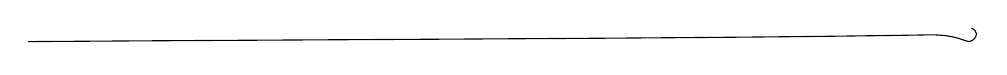
\begin{tikzpicture}[x=\linewidth,y=1mm,line cap=round]
\draw (0,0) .. controls (.35,.3) and (.72,.4) .. (.94,.85) .. controls (.98,1) and (.982,-.55) .. (.99,.25) .. controls (.994,.65) and (.995,1.35) .. (.988,1.7);
\end{tikzpicture}}}

\noindent * Research Fellow of the Atlas Computer Laboratory

\handwritten{\figure{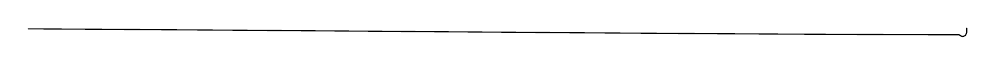
\begin{tikzpicture}[x=\linewidth,y=1mm,line cap=round]
\draw (0,.3) .. controls (.32,.08) and (.72,-.4) .. (.975,-.45) .. controls (.981,-1.05) and (.984,-.36) .. (.983,.38);
\end{tikzpicture}}}

\noindent 1. Introduction. This paper describes in general terms my attempts to extend and generalise congruence properties of modular forms with the aid of a computer(the ICT Atlas 1 computer of the Science Reserach Council at Chilton). The main practical conclusion can be stated simply: working in continuous direct contact with a large and powerful computer establishment has led to results far beyond my original expectations. Accordingly it seems worth while to try and give here some account of the actual process of discovery as it appeared to me at the time,which involves in effect a description of the work in reverse logical order; and to publish elsewhere the full mathematical details and a ``logical'' exposition based on the work in reverse order of time.

I have used Atlas to obtain a number of results,some of which are more interesting computationally than the present work. But in so far as the computer's function is to assist research,what matters is the final mathematical result rather than(to be fanciful) the machine's personal enjoyment of the tasks it has been ordered to perform. I am perfectly clear that the work described in this paper represents the most significant use I have made of Atlas. It might in theory have been possible to arrive at some of these results by \uline{a priori} reasoning; certainly the \unsure{.}cases where the proofs are complete require in the event no more computation than a few hours' hand work. But I would not myself have been able to conjecture the possibility of such results without the evidence provided by the computer.

I should like to thank the Director,Dr. J.Howlett,and my other colleagues at the Atlas Computer Laboratory for the frequent help they have given me. In particular I have had many valuable discussions

% archive sheet number: 40
\scanpage{42}
\noindent\hfill atkin \mspage{2}

\noindent with Dr. R.F.Churchhouse,both a number theorist and a veteran programmer,and Mr. \handwritten{E}.B.Fossey and Miss Barbara Stokoe have constantly assisted me with the Atlas Hartran(Fortran) system.

It is intended that this account shall be intelligible to the reader with no knowledge of modular theory\S{}\inserted{\handwritten{,}}\margin{\handwritten{\tikz[baseline=(cue.base)]{\node[inner sep=0pt] (cue) {\unsure{\S|$\delta$}};\draw (cue.south west) -- (cue.north east);}\ (comma)}}provided that he is prepared to accept that the coefficient \uline{$c(n)$} which we mainly consider is mathematically significant. However at some points we give brief additional explanations for the reader who has such knowledge.

\noindent\margin{\handwritten{/}}2. \uline{Ramanujan} \deleted{C}\uline{ongruences} \uline{for} \uline{primes} $q\handwritten{\leq}11$. The general theory of elliptic and modular functions had been in the process of development for about a century before RAMANUJAN(1919)conjectured his remarkable congruences for the partition function \uline{$p(n)$},defined combinatorially as the number of distinct ways of expressing \uline{$n$} as the sum of integral parts,where the order of the parts is immaterial. His conjecture was
\[
\handwritten{\text{\uline{if}}\quad 24n-1\equiv0\;(\text{\uline{mod}}\;5^{a}7^{b}11^{c})\quad
\text{\uline{then}}\quad p(n)\equiv0\;(\text{\uline{mod}}\;5^{a}7^{b}11^{c})}
\tag*{\handwritten{$\ldots$ (2.1)}}
\]
The curious appearance of $24n-1$ in \handwritten{(2.1)} is due to the fact that, writing
\[
\begin{aligned}
&\handwritten{x=e^{2\pi i\tau}\qquad (\,|x|<1,\ \mathrm{Im}\,\tau>0),}\\
&\handwritten{f(x)=(1-x)(1-x^{2})(1-x^{3})\ldots,}\\
\text{\deleted{we have}}\quad &\handwritten{\eta(\tau)=e^{\pi i\tau/12}f(x),}\\
\text{\inserted{\handwritten{we have}}}\quad &\handwritten{\sum_{n=0}^{\infty}p(n)\,x^{n}=1/f(x),}
\end{aligned}
\tag*{\handwritten{(2.2)}}
\]
and $\handwritten{\eta(\tau)}$ is a modular form of half-integral dimension and complicated multiplier system. Thus the congruence properties are naturally associated not with \uline{$f(x)$} whose reciprocal enumerates \uline{$p(n)$},but with \uline{$x^{1/24}f(x)$} ; that is,they are essentially modular and not combinatorial.$^{*}$ Ramanujan himself was of course well aware of this,

\noindent\handwritten{\rule{\linewidth}{0.4pt}}

\noindent\deleted{as his proofs}

\noindent *But see DYSON(19\handwritten{44}) and ATKIN and SWINNERTON-DYER(1954)for an exception.

\noindent\handwritten{\rule{\linewidth}{0.4pt}}

\noindent as his proofs of some particular cases show.

However this conjecture \handwritten{(2.1)},originally found from the

% archive sheet number: 41
\scanpage{43}
\noindent\hfill \unsure{a}\illegible{1}n \mspage{3}

\noindent evidence of hand computed tables,was found to fail for the case of $7^{3}$ by CHOWLA(1934) who observed that $p(243)$,computed by GUPTA(1935), is not divisible by $7^{3}$. This provides a simple illustration of the value of computers; had Ramanujan lived 50 years later he would surely have tested his conjecture extensively and probably found the correct form for $7$. WATSON(1938)proved the conjecture for all powers of $5$,and a suitably modified form for all powers of $7$,while ATKIN(1967)proved the conjecture for all powers of $11$. Thus the true form of \handwritten{(2.1)} is
\[
\begin{aligned}
&\handwritten{\text{\uline{if}}\quad 24n-1\equiv0\,(\text{\uline{mod}}\;5^{a}7^{b}11^{c})\quad
\text{\uline{then}}\quad p(n)\equiv0\,(\text{\uline{mod}}\;5^{a}7^{\beta}11^{c}),}\\
&\qquad\handwritten{\text{\uline{where}}\quad \beta=[(b+2)/2].}
\end{aligned}
\tag*{\handwritten{(2.3)}}
\]

It might be argued that for Ramanujan to have obtained the correct form \handwritten{(2.3)}would have been relatively unimportant; that the \uline{idea} of such a prop\rlap{\handwritten{\tikz[baseline=0pt,x=.7em,y=1ex,line cap=round]{\draw (-.18,-.82)--(.04,-.20)--(.45,-.78);\draw (.04,.4)--(.32,1.75);}}}\inserted{\handwritten{\uline{e}}}\margin{\handwritten{\tikz[x=.32em,y=.72ex,line cap=round]{\draw (0,0)--(1.2,3.4);\draw (.25,.68).. controls (.6,1.0) and (.8,.1) ..(1.2,.1);}}}rty is all that matters short of actual proof. But this is far from true in this kind of work,since the exact numerical form of such results can often provi\rlap{\handwritten{\tikz[baseline=0pt,x=1em,y=1ex]{\draw (0,-.35)--(.56,-.35)--(.56,1.7)--(1.06,1.7);}}}ed important clues as to a possible method of proof.

Despite the early recognition of the modular nature o\deleted{\unsure{n|f}}\handwritten{f} these congruences,it was not until 1949 that LEHNER(1949a,1949b) considered the analogous properties of $c(n)$,where
\[
\handwritten{j(\tau)=j(x)=\sum_{n=-1}^{\infty}c(n)\,x^{n}
=\left\{1+240\sum_{n=1}^{\infty}\sigma_{3}(n)x^{n}\right\}^{3}\big/xf^{24}(x)-744^{*}}
\tag*{\handwritten{$\ldots$ (2.4)}}
\]

\noindent\handwritten{\rule{\linewidth}{0.4pt}}

\noindent *We choose the arbitrary constant in $j(x)$ to make $c(0)=0$ and thus avoid tiresome exceptions to our results.

\handwritten{\figure{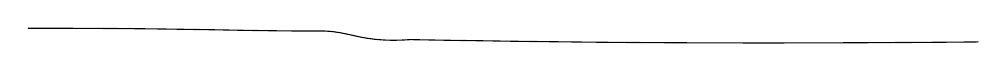
\begin{tikzpicture}[x=\linewidth,y=1mm,line cap=round]
\draw (0,.5) .. controls (.18,.5) and (.23,.1) .. (.31,.15) .. controls (.34,0) and (.35,-1.35) .. (.4,-.95) .. controls (.55,-1.25) and (.71,-1.55) .. (.995,-1.24);
\end{tikzpicture}}}

\[
\handwritten{\text{and}\qquad \sigma_{3}(n)=\sum_{d\mid n}d^{3}.}
\]

This function $j(\handwritten{\tau})$ is essentially the simplest of all modular forms, being in fact the Hauptmodul of the full modular group so that
\[
\handwritten{j\left(\frac{a\tau+b}{c\tau+d}\right)=j(\tau)\quad
\text{\uline{for} \uline{all} \uline{integral}}\quad a,b,c,d\quad
\text{\uline{with}}\quad ad-bc=1.}
\]
The results for $c(n)$ are
\[
\begin{aligned}
&\handwritten{\text{if}\quad n\equiv0\,(\mathrm{mod}\;2^{a}3^{b}5^{c}7^{d}11^{e})\quad
\text{then}\quad c(n)\equiv0\,(\mathrm{mod}\;2^{3a+8}3^{2b+3}\,\unsure{<|\hookleftarrow}}\\
&\hspace{4em}\handwritten{\unsure{>|\hookrightarrow}\,5^{c+1}7^{d}11^{e}).}
\end{aligned}
\tag*{\handwritten{(2.5)}}
\]

% archive sheet number: 42
\scanpage{44}
\noindent\hfill atkin \mspage{4}

\noindent These are all due to LEHNER(1949a,1949b,1950) except the cases \uline{$e$}$\handwritten{>}3$ due to ATKIN(1967). They represent what are perhaps the simplest and most natural ``Ramanujan-type'' congruences. The general possibilities are not confined to the coefficients \uline{$c(n)$} and \uline{$p(n)$},and many other modular forms have Fourier coefficients* with similar p\rlap{\handwritten{\tikz[baseline=0pt,x=1em,y=1ex]{\draw (0,-.35)--(.56,-.35)--(.56,1.7)--(1.06,1.7);}}}orperties. The work

\noindent\handwritten{\rule{\linewidth}{0.4pt}}

\noindent *That is,the coefficients of the expansion of a form $F(\handwritten{\tau})$ in powers of $x=\handwritten{e^{2\pi i\tau}}$.

\noindent\handwritten{\rule{\linewidth}{0.4pt}}

\noindent described in this paper was in fact conducted simultaneously with \uline{$c(n)$} and \uline{$p(n)$},the former being the simplest case and the latter an example\unsure{.} of the most difficult type of case; but we confine ourselves to \uline{$c(n)$} from now on in the present account.

\noindent 3. \uline{Congruences} \uline{for} $q=13$. It might have been hoped that results similar to \handwritten{(2.5)} would exist for primes $q\handwritten{>}11$,but this is(by now)extremely improbable(there are strong theoretical grounds for this assertion which is not merely based on the fact that no properties have been found).

\noindent The first results for $q\handwritten{>}11$,of an entirely different kind from those described in \handwritten{\S}2,are due to NEWMAN(1958),who proved that
\[
\handwritten{c(13^{2}n)\equiv8\,c(13n)\quad(\mathrm{mod}\;13),}
\tag*{\handwritten{(3.1)}}
\]
\[
\begin{aligned}
&\handwritten{\text{and}\quad\text{if}\quad t(n)=-c(13n)\quad\text{and}\quad p\ne13\quad\text{is prime then}}\\
&\qquad\handwritten{t(np)-t(n)t(p)+p^{11}\,t(n/p)\equiv0\,(\mathrm{mod}\;13).}
\end{aligned}
\tag*{\handwritten{$(3.2)^{*}$}}
\]

\noindent\handwritten{\rule{\linewidth}{0.4pt}}

\noindent *For any number-theoretic coefficient \uline{$t(n)$} we write $t(n)=0$ if \uline{$n$} is not an integer.

\noindent\handwritten{\rule{\linewidth}{0.4pt}}

From these Newman deduces,using the computed ``accident'' that $c(7\mathbin{.}13)\handwritten{\equiv}0\;(\mathrm{mod}\;13)$,that
\[
\handwritten{c(7\mathbin{.}13^{n})\equiv0\;(\mathrm{mod}\;13)\quad \text{if}\quad n\geq1}
\tag*{\handwritten{(3.3)}}
\]
\[
\handwritten{\text{and}\qquad c(91n)\equiv0\;(\mathrm{mod}\;13)\quad \text{if}\quad(n,7)=1.}
\tag*{\handwritten{(3.4)}}
\]
The first of these results shows that \uline{$c(n)$} is divisible by $13$ infinitely often; the second shows more,that \uline{$c(n)$} is divisible by $13$ in positive density of \uline{$n$}.

% archive sheet number: 43
\scanpage{45}
\noindent\hfill atkin \mspage{5}

Newman proves \handwritten{(3.2)} by observing that $t(n)\handwritten{\equiv\tau}(n)\;(\mathrm{mod}\;13)$, where* $\handwritten{\tau}(n)$ is defined by

\noindent\handwritten{\rule{\linewidth}{0.4pt}}

\noindent *We apologise to the reader for the two uses of $\handwritten{\tau}$. Both are well established, and there is no real danger of confusion.

\noindent\handwritten{\rule{\linewidth}{0.4pt}}

\[
\handwritten{\sum_{n=1}^{\infty}\tau(n)\,x^{n}=xf^{24}(x)}
\]

Now $\handwritten{\tau}(n)$ s\rlap{\handwritten{\tikz[baseline=0pt,x=1em,y=1ex]{\draw (0,-.35)--(.56,-.35)--(.56,1.7)--(1.06,1.7);}}}taisfies the \uline{identical} relation
\[
\handwritten{\tau(np)-\tau(n)\tau(p)+p^{11}\tau(n/p)=0}
\tag*{\handwritten{(3.5)}}
\]
as conjectured by RAMANUJAN(1916) and proved by MORDELL(1919),so that \handwritten{(3.1)} and \handwritten{(3.2)} are immediate. We may remark here that Ramanujan probably found this conjecture also by inspection of his own table of \deleted{e}\handwritten{\unsure{v|V}}alues of $\handwritten{\tau}(n)$ and his extraordinary intuition for algebraic form in this subject. It is a consequence of \handwritten{(3.5)} that $\handwritten{\tau}(n)$ is multiplicative,i.e.,
\[
\handwritten{\tau(mn)=\tau(m)\tau(n)\quad\text{if}\quad (m,n)=1.}
\tag*{\handwritten{(3.6)}}
\]

GLAISHER(\handwritten{1907}) had previously obtained a number of results similar to \handwritten{(3.6)} for coefficients relating to the expression of a number as sums of squares,but he did not obtain the crucial third term ( analogous to $p^{11}\handwritten{\tau}(n/p)$ in \handwritten{(3.5)})in his equations to obtain the full result similar to \handwritten{(3.5)}. Glaisher's results have been completed and fully proved by RANKIN(196\hspace{1em}).

% archive sheet number: 44
\scanpage{46}
\noindent\hfill atkin \deleted{5} \handwritten{\mspage{6}}

\noindent\deleted{\unsure{2|3}}\handwritten{3}.2. In 1962*O'Brien and I obtained a result which generalises

\noindent\handwritten{\rule{\linewidth}{0.4pt}}

\noindent *The results of \handwritten{\S}\deleted{\unsure{2|3}}\handwritten{3}.2 appear in ATKIN and O'BRIEN(1967). In the present context it seems natural to use real time.

\noindent\handwritten{\rule{\linewidth}{0.4pt}}

\noindent Newman's \handwritten{(3,1)}:
\[
\begin{aligned}
&\qquad\handwritten{\text{For all}\quad\alpha\geq1\quad\text{there exists a constant}\quad k_{\alpha}\quad\text{not diisible}}\\
&\handwritten{\text{by}\quad13\quad\text{such that for}\quad n\geq1\quad\text{we have}}\\
&\qquad\handwritten{c(13^{\alpha+1}n)\equiv k_{\alpha}\,c(13^{\alpha}n)\quad(\mathrm{mod}\;13^{\alpha}).}
\end{aligned}
\tag*{\handwritten{(3.7)}}
\]

\noindent Specifically,we had at this stage proved \handwritten{(3.7)} for $\alpha\handwritten{\leq}4$ by detailed hand computation using the irrational modular equation for $13$,and conjectured it for all $\alpha$ . It appeared to us at the time that the proof might depend on some very deep properties of certain numerical coefficients of the form $\handwritten{a_{i}\mathbin{.}13^{b_{i}}}$,and our subsequent proof of \handwritten{(\deleted{\unsure{2|6}}3,7)} for all $\alpha$ in 1963 arose from a fortunate numerical mistake. In fact one of us used \unsure{\textquotesingle}some incorrect values of the \uline{$a_{i}$} and still obtained \handwritten{(3,7)},suggesting that only the values of \uline{$b_{i}$} were relevant. This turned out to be the case. It thus appears that occasionally it is better \uline{not} to have a reliable computer; but this is the only instance I can quote from personal experience.

It is clear from \handwritten{(3.7)} that if we can find an ``accident'' of the form $c(13^{\alpha}n_{\unsure{0|o}})\handwritten{\equiv}0\;(\mathrm{mod}\;13^{\beta})$ for some $\beta\handwritten{\leq}\alpha$,then $c(13^{\alpha+n}n_{\unsure{0|o}})\handwritten{\equiv}0\;(\mathrm{mod}\;13^{\beta})$ for $n\handwritten{\geq}0$,so that \uline{$c(n)$} is divisible by $13^{\beta}$ infinitely often. After my appointment to Atlas in 1964 I computed \uline{$c(13^{6}n)$} modulo $13^{6}$ for $1\handwritten{\leq}n\handwritten{\leq}40960$ with output of the form
\diagram{$\begin{array}{ccc}
n & \qquad a(n)\qquad & b(n)
\end{array}$}
denoting that $c(13^{6}n)\handwritten{\equiv}a(n)\mathbin{.}13^{b(n)}\quad(\mathrm{mod}\;13^{6})$ ,with \uline{$a(n)$} prime to $13$. The largest $b(n)$ found was a disappointing $3$; there seemed a priori to be a reasonable chance of $4$ if the values of \uline{$c(13^{6}n)$} were random $(\mathrm{mod}\;13^{4})$ since $40960/\;13^{4}\handwritten{\bumpeq}1.4$. However an inspection of the results exposed some very interesting features. Thus $b(7)=$\ \parbox[c]{12mm}{\handwritten{\figure{\tikz[baseline=0pt,x=.28mm,y=.28mm,line cap=round]{\draw (0,0)..controls(5,6)and(9,6)..(12,2)..controls(19,-6)and(29,-6)..(37,6); \draw (1,.2)..controls(7,1.5)and(11,3)..(12,2); \draw (23,-2)..controls(30,-2)and(34,2)..(37,6);}}}}

% archive sheet number: 45
\scanpage{47}
\noindent\hfill atkin \deleted{6} \handwritten{\mspage{7}}

\noindent $=b(11)=1$,$b(77)=2$,and $b(154)=2$; also $b(757)=2$ and $b(5299=7\mathbin{.}757)=3$. We knew already from \handwritten{(3.2)} that if $(m,n)=1$ and $b(m)\handwritten{\geq}1$ then $b(mn)\handwritten{\geq}1$, but the above instances suggested immediately a multiplicative property modulo at least $13^{3}$. In fact a few further hand calculations using the values of $a(n)$ as well as $b(n)$ led us to the following conjecture:
\[
\begin{aligned}
&\text{\uline{Let}}\quad t(n)=c(13^{6}n).\quad \text{\uline{Then if}}\quad (m,n)=1\quad\text{\uline{we have}}\\
&\qquad t(1)t(mn)\handwritten{\equiv}t(m)t(n)\quad(\text{\uline{mod}}\;13^{6})\quad .
\end{aligned}
\tag*{\handwritten{(3.8)}}
\]

\noindent Since $c(13^{6})$ is prime to $13$,we may properly divide by it in the residue class ring modulo $13^{6}$; rewriting $t(n)=c(13^{6}n)/c(13^{6})$ we have \handwritten{(3.8)} with $t(1)=1$,and it was now natural to look for the precise detail analogous to \handwritten{(3.2)}. The natural power of $p$ in the third term is $p^{-1}$,and since $p^{11}\handwritten{\equiv}p^{-1}\;(\mathrm{mod}\;13)$ this agrees with \handwritten{(3,2)}. Thus finally,replacing $6$ by a general $\alpha$,we conjectured the following:
\[
\begin{aligned}
&\qquad\text{\uline{Let}}\quad\alpha\handwritten{\geq}1,\text{\uline{and}}\quad
p\handwritten{\ne}13\quad\text{\uline{be prime}. \uline{Then if}}\quad
t(n)=c(13^{\alpha}n\deleted{\unsure{-|=}}\handwritten{)}/c\handwritten{(}13^{\alpha}\deleted{\unsure{-|=}}\handwritten{)}\\
&\text{\uline{we} \uline{have}, \uline{for} \uline{all}}\quad n\handwritten{\geq}1\handwritten{,}\\
&\qquad t(np)-t(n)t(p)+p^{-1}t(n/p)\handwritten{\equiv}0\quad(\mathrm{mod}\;13^{\alpha})\deleted{\unsure{8|\beta}}\,.
\end{aligned}
\tag*{\handwritten{(3.9)}}
\]
\margin{\handwritten{/\deleted{8}}}

This conjec\rlap{\handwritten{\tikz[baseline=0pt,x=1em,y=1ex]{\draw (0,-.35)--(.56,-.35)--(.56,1.7)--(1.06,1.7);}}}utre I tested successfully on Atlas for $\alpha\handwritten{\leq}8$, $p\handwritten{\leq}97$,and $pn\handwritten{\leq}1000$,and have recently proved in general. We may now regard \handwritten{(3.7)} as the ramified form which \handwritten{(3.9)} takes for the exceptional prime $p=13$,and in fact we can rewrite \handwritten{(3.7)} as
\[
t(13n)\mathrel{\rlap{\raisebox{-.12ex}{\handwritten{\rule{.65em}{.55pt}}}}=}t(13)t(n)\quad(\mathrm{mod}\;13^{\alpha}).
\tag*{\handwritten{(3.10)\tikz[baseline=0pt,x=.18em,y=.6ex]{\fill (0,0) circle (.13);\fill (.65,.8) circle (.13);}}}
\]
We shall \deleted{\unsure{n|m}}in future refer to multiplicative co\deleted{m}\inserted{\handwritten{n}}\margin{\handwritten{/}}gruence properties similar to \handwritten{(3.9)} as M-results,and to their ramified cases similar to \handwritten{(3.10)} as R-results.

Now it is easy to show\rlap{\handwritten{\tikz[baseline=-.2ex,x=.3em,y=.65ex,line cap=round]{\draw (0,0)--(1.2,3.3);\draw (.36,.84)--(.97,.84).. controls (.92,.42) and (1.0,.17)..(1.12,.1);}}}\inserted{\handwritten{from (3.2)}}\margin{\handwritten{\tikz[baseline=-.2ex,x=.3em,y=.65ex,line cap=round]{\draw (0,0)--(1.2,3.3);\draw (.36,.84)--(.97,.84).. controls (.92,.42) and (1.0,.17)..(1.12,.1);}}} by the theory of second order linear difference equations that for each $p\handwritten{\ne}13$ there exists some $\theta$ such that $c(13\mathbin{.}p^{\theta})\handwritten{\equiv}0\;(\mathrm{mod}\;13)$. Thus from \handwritten{(3.9)} we have for \unsure{a}ny $\alpha\handwritten{\geq}1$ the result
\[
\handwritten{c(13^{\alpha}\mathbin{.}P\mathbin{.}n)\equiv0\;(\mathrm{mod}\;13^{\alpha})\quad\text{\uline{if}}\quad(n,P)=1}
\tag*{\handwritten{(3\unsure{,.|..}11)}}
\]

% archive sheet number: 46
\scanpage{48}
\noindent\hfill atkin \mspage{8}

\[
\text{where}\quad\mathrm{P}=\handwritten{\prod_{i=1}^{\alpha}p_i^{\theta_i},}
\]
\noindent so that(since there are infinitely many primes) \uline{$c(n)$} is divisible by $13^{\alpha}$ in positive density of $n$ for every $\alpha\handwritten{\geq}1$. Hence in the final analysis the extensive computation of $c(13^{\handwritten{6}}n)$ becomes unnecessary \deleted{\uline{for}}\unsure{.} but without it we could not have found \handwritten{(3.9)}.

However in this connection there is a subtle difference in the corresponding work for \uline{$p(n)$},and generally for the Fourier coefficients of forms of half-integral dimension. In these cases there are results of M- and R-type,but they contain an unknown constant which is not a value of the coefficient,and one cannot prove the existence of ``accidents'' by the use of difference equations for a general prime $p\handwritten{\ne}13$. Thus in order to prove that \uline{$p(n)$} is divisible by $13^{\alpha}$ in positive density of \uline{$n$} it is necessary to compute $\alpha$ accidents,even though the \uline{general} M-result is proved \deleted{\uline{for all}} $\handwritten{\alpha}$.\margin{\handwritten{\tikz[baseline=0pt,x=.3em,y=.4ex,line cap=round]{\draw (.75,3.9)..controls(.8,3.15)and(.1,3.3)..(.2,2.6)..controls(.3,2.05)and(1,2.4)..(.72,2.8)..controls(.4,3.1)and(.25,1.8)..(.7,1.55)..controls(1.05,1.25)and(.45,.9)..(.28,1.3);\draw(.05,-.6)--(.83,4.1);}}} I have in fact found 13 such accidents,so that \uline{$p(n)$} is divisible by $13^{13}$ in positive density of $n$. (The second ``13'' is of course an irrelevant accident!)

\noindent \deleted{\unsure{1|4}}\handwritten{4}. \uline{The} \uline{cases} $q=17,19$,\uline{and} $23$. Concurrently with the work for $\uline{q}=13$ described in the last section,the methods of ATKIN(1967) were used to obtain suitable systems of modular functions for the primes $\uline{q}=17,19,23,29,31$,and $37$,with a view to obtaining \deleted{\unsure{p)|p}} \margin{\handwritten{\tikz[baseline=0pt,x=.35em,y=.4ex,line cap=round]{\draw (.45,3.8)..controls(.42,3.1)and(-.05,3.15)..(.02,2.5)..controls(.08,2)and(.64,2.2)..(.52,2.7)..controls(.44,2.95)and(.03,1.8)..(.4,1.5)..controls(.75,1.15)and(.25,.9)..(.1,1.3);\draw(.15,-.5)--(1.45,3.8);}}}R-results. As soon as the M-results for 13 appeared,it required no additional personal effort(and in fact very little machine time)to test the situation on these primes with regard to M-results. I found that the conjectures \handwritten{(3.9)} and \handwritten{(3.10)} held for $\uline{q}=17,19$,and $23$,word for word but replacing 13 by \uline{$q$}. This provides a further illustration of the value of \handwritten{a} computer: with the necessary subroutines already written one can multiply instances without the loss of momentum which hand calculation would involve. There was in this case no particular reason to expect ``the same again''; the type of modular equation for $\uline{q}=13$ does not exist for $\uline{q}>13$\unsure{,|.}

% archive sheet number: 47
\scanpage{49}
\begin{flushright}
atkin \mspage{\unsure{9|8|6}}
\end{flushright}

However a significant difference arose here as to the proof of these M- and R-results. If we define for any power series
\[
\handwritten{A(x)=\sum_{n\geqslant N}a(n)x^{n}}
\]
the operator $U=U_{q}$ by
\[
\handwritten{U A(x)=\sum_{qn\geqslant N}a(qn)x^{n},}
\]
then we have
\[
\handwritten{\sum_{n=1}^{\infty}c(q^{\alpha}n)x^{n}=U^{\alpha}j(x).}
\]

As a specific example we now take the simplest case \uline{$q$}$=19$. We can show by modular theory* that there exist functions $g_{n}(x)$ for $n\handwritten{\geqslant}1$
\par\noindent\rule{\linewidth}{0.3pt}\par
\noindent *Of course the same theory could have been applied to the case $q=13$.The main difficulty is that this comparatively deep theory gives for our present purposes results which are \uline{weaker} than those obtained from an elementary use of the modular equation for $q=13$.
\par\noindent\rule{\linewidth}{0.3pt}\par
\noindent with integral coefficients\inserted{ in their power series expansions} and leading terms $x^{n}$,such that
\[
\resizebox{.86\linewidth}{!}{$\displaystyle \handwritten{\begin{aligned}[b]
 U_{19}\,j(x)&\equiv a_{1}\,g_{1}(x)+19\,a_{2}\,g_{2}(x)+19\,a_{3}\,g_{3}(x)\quad(\mathrm{mod}\;19^{2}),\\
 U_{19}\,g_{1}(x)&\equiv c_{11}\,g_{1}(x)+19\,c_{12}\,g_{2}(x)+19\,c_{13}\,g_{3}(x)\quad(\mathrm{mod}\;19^{2}),\\
 U_{19}\,g_{2}(x)&\equiv c_{21}\,g_{1}(x)+c_{22}\,g_{2}(x)+c_{23}\,g_{3}(x)+\\
 &\hspace{13em}+19\,c_{24}\,g_{4}(x)\quad(\mathrm{mod}\;19^{2}),\\
 \text{\deleted{\unsure{etc.,|etc,}}}\quad\vdots&
\end{aligned}}$}
\tag*{\handwritten{(4.1)}}
\]
\reversemarginpar\margin{\handwritten{\tikz[x=1em,y=1em,baseline=-.15em]{\draw (.57,.8)--(.07,-.7); \draw (.44,.51) .. controls (.07,.69) and (.04,.31) .. (.24,.24) .. controls (.02,.18) and (.03,.01) .. (.33,.03);}}}
where the \inserted{\handwritten{$a_{i}$ and}} $\handwritten{c_{ij}}$ are integral constants. Now it turns out \uline{by} \uline{actual} \uline{computation} that some of these constants contain powers of $19$ which were not deducible \uline{a} \uline{prio\mbox{\makebox[0pt][l]{\handwritten{\tikz[x=1em,y=1ex,baseline=0pt]{\draw (.02,-.28)--(.54,-.28)--(.54,1.54)--(1.01,1.6);}}}ir}}; moreover these full powers of $19$ which occur in actual fact are needed to prove the M- and R\normalmarginpar\margin{\handwritten{\tikz[x=1em,y=1em,baseline=-.1em]{\draw (.5,.72)--(.08,-.35) (.27,-.10)--(.38,-.35);} $-$\\(hyphen)}}\deleted{j}\inserted{\handwritten{-}}results. Thus in these cases(\uline{$q$}$=17,19,\text{and }23$)we have at present the situation that the M- and R-results can only be established for a limited number of
% archive sheet number: 48
\scanpage{50}
\begin{flushright}
at\illegible{1} \mspage{10}
\end{flushright}

\noindent fixed values of $\alpha$,and that even these limited results depend on computation beyond any reasonable prospect of hand calculation(except for $\unsure{\alpha|a}=1$). However in view of the complete test of the M-results the prggrams can be regarded as self-checking,since the M\margin{\handwritten{\tikz[x=1em,y=1em,baseline=-.1em]{\draw (.5,.72)--(.08,-.35) (.27,-.10)--(.38,-.35);} $-$\\(hyphen)}}\deleted{\unsure{j|;|,}}\inserted{\handwritten{-}}results follow theoretically from the independently computed values of $\handwritten{c_{ij}}$ in \handwritten{(4.1)} .

Since the subgroups $\handwritten{\Gamma_{0}}(13)$, $\handwritten{\Gamma_{0}}(17)$, $\handwritten{\Gamma_{0}}(19)$,and $\handwritten{\Gamma_{0}}(23)$ of the modular group have genera $0,1,1,\text{and }2$ respectively,it is remarkable that all these primes should exhibit the same behaviour with regard to our multiplicative congrue\makebox[0pt][l]{\handwritten{\tikz[x=1em,y=1ex,baseline=0pt]{\draw (.02,-.28)--(.54,-.28)--(.54,1.54)--(1.01,1.6);}}}cne p\makebox[0pt][l]{\handwritten{\tikz[x=1em,y=1ex,baseline=0pt]{\draw (.02,-.28)--(.54,-.28)--(.54,1.54)--(1.01,1.6);}}}orperties. It thus seems possible that some entirely different method or theory may exist which would give an uniform proof of all these cases.

\deleted{4}\handwritten{5}. \uline{The} \uline{cases} $q\handwritten{\geqslant}29$. As the reader may have anticipated from the non-appearance of $29$ in \handwritten{\S\,4},the direct analogy to \handwritten{(3.9)} and \handwritten{(3.10)} breaks down for $q=29$. Considering first the R-results modulo $29$ only,we can prove by the combination of modular theory and computing described in \handwritten{\S}\deleted{\unsure{3|5}}\handwritten{4} that
\[
\handwritten{\begin{aligned}
U_{29}\,j(x)&\equiv a_{1}\,g_{1}(x)+a_{2}\,g_{2}(x)\quad(\mathrm{mod}\;29),\\
U_{29}\,g_{1}(x)&\equiv 26\,g_{1}(x)+14\,g_{2}(x)\quad(\mathrm{mod}\;29),\\
U_{29}\,g_{2}(x)&\equiv 3\,g_{1}(x)+21\,g_{2}(x)\quad(\mathrm{mod}\;29).
\end{aligned}}
\]
Thus
\[
\resizebox{\linewidth}{!}{$\displaystyle \handwritten{U_{29}\{g_{1}(x)+\mu\,g_{2}(x)\}\equiv(3\mu-3)\,g_{1}(x)+(14-8\mu)\,g_{2}(x)\quad(\mathrm{mod}\;29),}$}
\]
and if we attempt to make the RHS a multiple of $\handwritten{\{}g_{\handwritten{1}}(x)\ \deleted{\unsure{\text{and }g_{2}|\text{and }\mu_{2}}}\handwritten{{}+\mu\,g_{2}(x)\}}$ we are led to the congruence
\[
\handwritten{\mu^{2}-8\mu+5\equiv 0\;(\mathrm{mod}\;29)}
\]
which has in fact no roots. However if we now consider our various coefficients \inserted{\handwritten{not}} as integers modulo $29$,but as elements of the Galois field $\mathrm{GF}(29^{2})$ we may assert(using ``$=$'' rather than ``$\handwritten{\equiv}$'' in a field of characteristic $29$):
\normalmarginpar
% archive sheet number: 49
\scanpage{51}
\begin{flushright}
atkin \mspage{11}
\end{flushright}

\[
c(29n)=a\,\handwritten{\lambda}(n)+\mathord{\rlap{$\handwritten{\bar{\phantom{a}}}$}a}\,\handwritten{\bar{\lambda}}(n),
\]
\uline{where} $a,\ \handwritten{\lambda}(n)$,\uline{and} \uline{their} \uline{conjugates} $\mathord{\rlap{$\handwritten{\bar{\phantom{a}}}$}a},\ \handwritten{\bar{\lambda}}(n)$ \uline{lie} \uline{in} $\rlap{\smash{\handwritten{\tikz[x=1em,y=1ex,baseline=0pt]{\draw (.09,-.42) .. controls (.48,-.71) and (.92,-.63) .. (1.1,-.28); \draw (.16,-.94)--(.20,-.67) (.03,1.17)--(.20,1.47); \node[inner sep=0pt] at (.87,1.95){\tiny\unsure{?}}; \draw (1.17,2.20)--(1.30,2.58);}}}}\unsure{\mathbb{GF}|\mathrm{GF}}(29^{2})$,\margin{\handwritten{\tikz[baseline=(f.base)]{\node[inner sep=1.5pt](f){$GF$};\draw (f.center) ellipse [x radius=1.12em,y radius=.78em];}}}
\[
\text{\uline{and} }\handwritten{\lambda}(29n)=\handwritten{\lambda}(29)\handwritten{\lambda}(n)\ ,\
\handwritten{\bar{\lambda}}(29n)=\handwritten{\bar{\lambda}}(29)\handwritten{\bar{\lambda}}(n).
\tag*{(5.2)}
\]

Of course $c(29n)$ itself lies in $\mathrm{GF}(29)$. We may infer from (5.2) that \handwritten{,} for all $n\handwritten{\geqslant}1$\handwritten{,}
\[
c(29^{29^{2}}n)\handwritten{\equiv}c(29n)\qquad(\mathrm{mod}\;29).
\]
We have also an M-result for $\handwritten{\lambda}(n)$ of the usual kind:
\[
\handwritten{\lambda}(np)-\handwritten{\lambda}(n)\handwritten{\lambda}(p)+p^{-1}\handwritten{\lambda}(n/p)=0\quad\text{\uline{if} }p\mathrel{\rlap{$\handwritten{/}$}=}29.
\tag*{(5.3)}
\]

It is now quite \unsure{éasy|easy} to foresee the natural general conjecture for powers of $\unsure{29'|29}$ in the form:

\uline{For} \uline{all} $\alpha\handwritten{\geqslant}1$ \uline{we} \uline{have} \handwritten{\tikz[x=1em,y=1em,baseline=0pt]{\draw (0,.45)--(.14,.49);}}
\[
c(29^{\alpha}n)=a\,\handwritten{\lambda}(n)+\mathord{\rlap{$\handwritten{\bar{\phantom{a}}}$}a}\,\handwritten{\bar{\lambda}}(n),
\]
\uline{where} $a,\handwritten{\lambda}(n)$,\uline{and their conjugates} $\mathord{\rlap{$\handwritten{\bar{\phantom{a}}}$}a},\handwritten{\bar{\lambda}}(n)$,\uline{lie in an} \uline{extension} \uline{of} \uline{the} \uline{residue} \uline{class} \uline{ring} \uline{modulo} $29^{\alpha}$ \uline{defined} \uline{by} \uline{an} \uline{irreducible} \uline{quadratic} \uline{equation},\uline{and} \uline{for} $n\handwritten{\geqslant}1$ \uline{we} \uline{have}
\[
\resizebox{.86\linewidth}{!}{$\displaystyle \begin{aligned}[b]
&\handwritten{\lambda}(29n)=\handwritten{\lambda}(29)\handwritten{\lambda}(n)\\
\text{\uline{and} }\;&\handwritten{\lambda}(np)-\handwritten{\lambda}(n)\handwritten{\lambda}(p)+p^{-1}\handwritten{\lambda}(n/p)=0\quad\text{if }p\mathrel{\rlap{$\handwritten{/}$}=}29.
\end{aligned}$}
\tag*{(5.4)}
\]

This is subject to the same reservations as the cases $q=17,19,\text{and }23$; it is only proved for $\alpha\handwritten{\leqslant}5$,and then only by a combination of modular theory and computation.

The case $q=31$ is precisely analogous to $q=29$,while for $q=37$ we find that \uline{three} conjugates are required over an extension of the ring modulo $37^{\alpha}$ defined by an irreducible \uline{cubic} \tikz[x=1em,y=1em,baseline=0pt]{\fill (.03,.34) circle[radius=.028];} equation.At this point it seemed unprofitable to compute any further cases in detail, since no essentially new features arose after $29$. However brief pre\inserted{\handwritten{l}}iminary investigations for all primes \uline{$q$} with $41\handwritten{\leqslant}q\handwritten{\leqslant}67$ suggest that in general $c(q^{\alpha}n)$ will be a linear combination of $\handwritten{[}q/12\handwritten{]}$ \inserted{\handwritten{multiplicative}} coefficients lying in various extensions of the ring modulo $q^{\alpha}$. In addition the analogy with Hecke theory for modular forms of negative dimension
% archive sheet number: 50
\scanpage{52}
\begin{flushright}
atkin \mspage{12}
\end{flushright}

\noindent which we now discuss \unsure{bríefly|briefly} in \handwritten{\S}\,6 below indicates that (5.4) is the right kind of property to generalise for all \uline{$q$}.

6. \uline{The} \uline{analogy} \uline{with} \uline{Hecke} \uline{theory}. We now return to the exact multiplicative properties such as (3.5). These have been extensively generalised by Hecke,Petersson,and others; for a useful summary we refer to RANKIN(196\hspace{.6em}). As a particular example of the theory we take the case of
\[
\handwritten{\sum_{n=2}^{\infty}}t_{2}(n)x^{n}=x^{2}f^{48}(x),
\]
for which Hecke showed that
\[
t_{2}(n)=a\,\handwritten{\lambda}(n)+\mathord{\rlap{$\handwritten{\bar{\phantom{a}}}$}a}\,\handwritten{\bar{\lambda}}(n),
\]
where $a,\handwritten{\lambda}(n)$,and their conjugates $\mathord{\rlap{$\handwritten{\bar{\phantom{a}}}$}a},\handwritten{\bar{\lambda}}(n)$ lie in the quadratic field $\deleted{\unsure{q|Q}}$\reversemarginpar\margin{\handwritten{\tikz[x=1em,y=1em,baseline=-.1em]{\draw (.56,.7)--(.03,-.53) (.78,.39)--(.20,-.74); \draw (.33,.39) .. controls (.13,.46) and (.14,.16) .. (.27,.04) .. controls (.4,-.11) and (.26,-.26) .. (.25,-.3);}}} $Q(\handwritten{\surd}\,144169)$,and for $n\handwritten{\geqslant}1$ and prime $p$ we have
\[
\handwritten{\lambda}(np)-\handwritten{\lambda}(n)\handwritten{\lambda}(p)+p^{23}\handwritten{\lambda}(n/p)=0.
\tag*{(6.1)}
\]

It seems clear that the multiplicative congruence properties we have described in terms of extensions of residue class rings are closely anal\deleted{g}\inserted{\handwritten{\unsure{a|u|o}}}gous to the exact multiplicative properties of Hecke theory in terms of algebraic number fields. We have not described in this account the underlying common feature of the Hecke operators,but it seems reasonable to conjecture that some kind of ``$\handwritten{\mathfrak{p}}$-adic'' Hecke theory\normalmarginpar\margin{\handwritten{$\left(\begin{gathered}\text{German}\\[-.4ex]p\end{gathered}\right)$}} exists for modular forms of positive and(as for $c(n)$) zero dimension, which is a counterpart of the exact theory for forms of negative dimension. The present difficulties in the way of precise formulation and proof see\inserted{\handwritten{m}} formidable in so far as the \uline{congruences} we have considered in this paper arise essentially at just one point($\inserted{\handwritten{\tau=}}i\handwritten{\infty}$) of the complex upper half-plane,whereas the \uline{identities} of Hecke theory exist at all points of the upper half-plane,taking the form of multiplicative properties for Fourier coefficients at $\inserted{\handwritten{\tau=}}i\handwritten{\infty}$.

7. \uline{Non-Ramanujan} \uline{congruences} \uline{for} \uline{primes} $q\handwritten{\leqslant}11$. Once the above properties for primes $q\handwritten{\geqslant}13$ had been found it was clear that something similar must
% archive sheet number: 51
